
\documentclass[10pt,journal,compsoc]{IEEEtran}

\usepackage{graphicx}





\ifCLASSOPTIONcompsoc
  
  \usepackage[nocompress]{cite}
\else

  \usepackage{cite}
\fi






\ifCLASSINFOpdf

\else

\fi



\hyphenation{op-tical net-works semi-conduc-tor}


\begin{document}

\title{Cloud Computing\\ Characteristics,Security Issues and Data Protection}


\author{Sarabjeet~Kumar,~\IEEEmembership{~RESEARCH METHODS IN COMPUTING AND IT  - GMIT ,}
        \IEEEmembership\\{}
       G00305450 \IEEEmembership \\{ ~ Professor -  Dr Martin Kenirons }% <-this % stops a space
\IEEEcompsocitemizethanks{


\IEEEcompsocthanksitem }
}


\markboth{Journal of Secure Cloud Computing , November 2016}
{Shell \MakeLowercase{\textit{et al.}}}

\IEEEtitleabstractindextext{
\begin{abstract}
In this paper, the author focuses on Cloud Computing which can be described as a distributed architecture integrating computer servers and other resources on a scalable platform providing on demand computing resources and services. The author provides a definition of cloud computing, the various cloud deployment and service delivery models, and the main security risks and data protection issues that are present within the cloud computing industry.
\end{abstract}

% Note that keywords are not normally used for peerreview papers.
\begin{IEEEkeywords}
cloud computing, characteristics deployment models,service delivery models, Iaas, Saas, PaaS, Security issues, data protection
\end{IEEEkeywords}}


\maketitle

\IEEEdisplaynontitleabstractindextext

\IEEEpeerreviewmaketitle



\IEEEraisesectionheading{\section{Introduction}\label{sec:introduction}}



\IEEEPARstart{I}{}n the past few years Cloud computing has emerged as the new model for hosting and delivering services over the Internet.  As indicated in [1] Cloud computing groups’ together computer servers and other resources usually offering customers combined capacity on an on-demand, pay-per-cycle basis.


\hfill 
 
\hfill 

\vspace{2mm}
In the field assert that Cloud computing relates to both the applications delivered as services over the Internet and the hardware and systems software in the data centers that provide those services [2]. Cloud computing allows a company to increase its capacity and capabilities without having to invest in new infrastructure, personnel training, or licensing of new software [3]. However in today’s evolving IT world with more information in relation to individuals and companies being placed in the cloud security concerns about the safety of a Cloud Computing environment is currently a hot topic. In this literature review the author will give an overview of Cloud Computing including a definition, its characteristics, service delivery models, its architecture and security issues relating to its infrastructure. 

\subsection{CLOUD COMPUTING DEFINITION}
The word "cloud" originated in the telecommunications industry when providers began using virtual private network (VPN) services for data communications. Cloud computing is associated with computation, software, data access and storage services and moves computing and data away from desktop and portable PCs into large data centers [4].

\vspace{2mm}
According to the National Institute of Standards and Technology Cloud computing can be defined as "a model for enabling convenient, on-demand network access to a shared pool of configurable computing resources (e.g., networks, servers, storage, applications, and services) that can be rapidly provisioned and released with minimal management effort or service provider interaction" [5]. 

\vspace{2mm}
Other academics define the term as “a set of network enabled services, providing scalable, QoS guaranteed, normally personalized, inexpensive computing infrastructures on demand, which could be accessed in a simple and pervasive way” [6]. Cloud computing is TCP/IP based and integrates computer technologies such as fast micro processor, vast memory, high-speed network and reliable system architecture [7]. Although Cloud Computing is not a new innovative technology, it is a new operations model that brings together a set of existing technologies thereby changing the way industries and firms conduct businesses by making them more efficient, user friendly and profitable.  Many believe that the role of Cloud computing is to make better use of resources by combining them to achieve higher output and solve large scale computation problems [8].

\vspace{2mm}
Cloud computing utilises a service-driven business model with hardware and platform-level resources provided as services on an on-demand basis [9]. It is modelled on a “pay as you system, which allows businesses to pay for only the service they use thereby making it an attractive option for those firms which cannot afford buying, installing and maintaining the required services [10]. 


\subsection{CHARACTERISTICS OF CLOUD COMPUTING} 
\vspace{2mm}
Flexibility/Elasticity: users can access computing resources quickly to scale out or up. 

\vspace{2mm
}Scalability of infrastructure: new nodes or physical servers can be added or removed from the network with limited 	modifications to set up and software thus the behaviour of one part hardly affects other parts.

\vspace{2mm}
Broad network access: capabilities are available over the network and can be accessed through standard and used through various platforms (e.g., mobile phones, laptops, and PDAs). 

\vspace{2mm}
Economies of scale and cost effectiveness: Cloud computing deployments tend to be as large as possible in order to take advantage of economies of scale and deployments can often be located close to cheap power stations and in low-priced real 	   estate, to lower costs [11]. 

\vspace{2mm}
TCP/IP: this gives reliable delivery connecting between remote applications. TCP/IP is widely used in cloud computing and the HTTP protocol over TCP/IP supports the user experience by establishing trust and security [7].

\vspace{2mm}
Ease of use: most cloud computing providers use interfaces which are simpler than other application program interfaces (API) and allows users to access or share information from anywhere at any time [12]. 


\subsection{CLOUD DEPLOYMENT MODELS}
\vspace{2mm}
Organisations must decide on the type of cloud to be utilised and can choose from a public, private, hybrid or community cloud depending on which deployment meets their needs:

\subsubsection{ Private Cloud}
\vspace{2mm}
This is set up within an organization’s internal enterprise data center and all cloud resources and applications are managed by the organization itself, similar to that of an Intranet [13]. The cloud infrastructure can be managed by the organisation or a third party existing on/off the premises. Only the organization and designated stakeholders have access to operate on a specific Private cloud thus making it easier to manage security, maintenance and upgrades while also providing more control over the deployment and use [8].

\subsubsection{Public Cloud}
\vspace{2mm}
The type of cloud infrastructure is made available to the general public or a large industry group and is owned by an organisation selling cloud services [11]. It allows users' access to the cloud via interfaces using web browsers and users pay only for the time duration they use the service, thus reducing the operation costs on IT expenditure [8]. As asserted in [13] Public clouds are less secure than other cloud models as they are more prone to malicious attacks.

\subsubsection{Community Cloud}
\vspace{2mm}
A community cloud is described as being organised to serve a common function or purpose and may be for one or more organisations’ as they share common features such as their mission, policies, security, or regulatory compliance needs [14]. A community cloud may be managed by the organisations or by third party providers. An example is Unilever that connects employee communities from around the world to internal marketing teams with external partners and agencies that allows for collaboration and sharing of resources [15].

\subsubsection{Hybrid Cloud}
\vspace{2mm}
A hybrid cloud can be described as a private cloud linked to one or more external public cloud services, managed centrally through a secure network [16]. It allows organisations to serve its needs in the private cloud and if needed requests the public cloud for computing resources [16].  In choosing a cloud deployment model organisations need to assess the security concerns in relation to each model carefully to decide which would best suit the needs of the business.

\subsubsection{SERVICE DELIVERY MODELS}
\vspace{2mm}
The architecture of Cloud computing can be categorised according to the three types of delivery models: software as a service (SaaS), platform as a service (PaaS), and infrastructure as a service (IaaS). As can be seen from the figure below the cloud environment can be divided into 4 layers: the hardware/data center layer, the infrastructure layer, the platform layer and the application layer.



\subsection{Cloud computing architecture [9]}
\vspace{2mm}

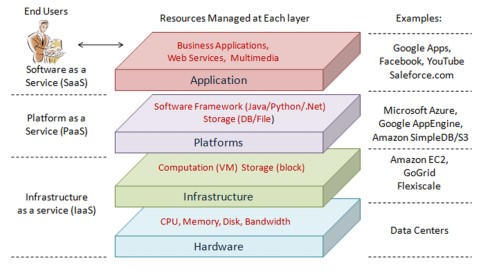
\includegraphics[height=7cm,width=9cm]{cloudCompArch.jpg}





\subsubsection{IaaS}
\vspace{2mm}
Infrastructure as a Service is a form of hosting which encompasses network access, routing services and storage based on virtualisation technology [17]. Users acquire computing resources such as processing power, memory and storage from an IaaS provider, with the provider supplying the hardware and administrative services needed to store applications and a platform for running applications. The data operational centre is managed by the IaaS provider and users deploy and manage the software services themselves. Furthermore the client does not purchase the required servers, data center or the network resources and pays only for the time duration they use the service thus allowing them to achieve a much faster service delivery with less cost. Examples of IaaS include GoGrid, Flexiscale, Layered Technologies, Joyent, Amazon Web Services Elastic Compute Cloud (EC2), Secure Storage Service (S3) and Mosso/Rackspace [17].

\subsubsection{PaaS}
\vspace{2mm}
Platform-as-a-Service provides developers with a platform including all the systems and environments that support the complete life cycle of building and delivering web applications and services available from the Internet [18]. It is a method to rent hardware, operating systems, storage and network capacity over the internet and allows customers to utilise these services without the cost of buying and managing the required infrastructure. It consists of infrastructure software including a database, middleware and development tools with a virtualized and clustered grid computing architecture often the foundation for this infrastructure software [1]. Google AppEngine allows developers to write in Python or Java, other examples of PaaS include Facebook F8, Salesforge App Exchange and Amazon EC2.


\subsubsection{PaaS}
\vspace{2mm}
SaaS providers host and manage certain applications in their own data centers and make them available to users over the internet thereby eliminating the need to install and run applications on the users system [1]. Customers can remotely access the software through the Internet with a usage-based pricing model. For example Salesforce is a successful leader in providing online CRM (Customer Relationship Management) Services, Live Mesh by Microsoft allows files and folders to be shared and synchronized across multiple devices [19]. Although PaaS and SaaS sound similar it should be noted that they are different in terms of what they provide customers; SaaS hosts completed cloud applications whereas PaaS offers a development platform that hosts both completed and in-progress cloud applications [20].


\subsection{ADVANTAGES OF CLOUD COMPUTING}

\vspace{2mm}
Cloud computing offer users many advantages including:

\vspace{2mm}
Cost- users of the technology only pay per usage of time, storage and services thus reducing the cost of owning the infrastructure. 

\vspace{2mm}
Performance- as there is a large network of high powered computers with high processing power the performance level is improved. 

\vspace{2mm}
Consistently upgraded-the cloud network infrastructure is maintained and upgraded by the cloud service provider. 

\vspace{2mm}
Scalability- the user can request to increase or reduce requirements depending on the user’s needs. 

\vspace{2mm}
Environmentally friendly- due to resource sharing users do not need to avail of their own large data centres thereby reducing the consumption of power. 

\vspace{2mm}
Mobility- users can access their information/documents anywhere in the world. 

\vspace{2mm}
Increased Storage Capacity- as Cloud computing has many networks in the Cloud the amount of storage available to users is increased [21], [22], [23], [24], [25].

\subsection{DISADVANTAGES OF CLOUD COMPUTING }

\vspace{2mm}
There are certain security threats and issues of implementing Cloud computing: 

\vspace{2mm}
Loss of data- users are responsible for the security of their data unless they protect it through internal or external data protection measures or simply not backing up their data can incur loss. 

\vspace{2mm}
Hijacking- due to the sophistication and the occurrence of more attacks online, hijacking probability is increased. 

\vspace{2mm}
Loss of control over the process- as Cloud computing encompasses providers allowing users access to these resources and infrastructure, less control is available unless a private Cloud is implemented. 

\vspace{2mm}
Insider attacks- a dishonest or fraudulent employee may steal or corrupt data. 


\vspace{2mm}
Legal aspects- if there is no Service Level Agreements (SLA) in place, the user may not be able to claim against the cloud service provider. Another issue is the jurisdiction if different continents are involved in a dispute, which country’s legislation applies?  [21], [23], [24], [26], [27], [28].


\subsection{CLOUD COMPUTING SECURITY ISSUES}
\vspace{2mm}

Although Cloud computing provides customers many benefits, there are many issues concerning security that affect customers and service providers. Privacy is not only important for business but also individual users of the 	Cloud e.g. an individual’s personal information or a company’s sensitive information such as customer credit/debit card details. Below are examples of the different security issues that may affect Cloud computing users/providers:

\vspace{2mm}
\subsubsection{IP Spoofing}
Spoofing involves creating TCP/IP packets using somebody else’s IP address whereby the intruder gains unauthorized access and sends messages to a computer with an IP address indicating that the message is coming from a trusted host [29], [30]. IP spoofing’s main aim is to gain unauthorized access to a computer. There are many variations on the types of attacks that successfully employ IP spoofing.


\vspace{2mm}
\subsubsection{Denial of Service Attack (DoS)}
A DoS attack occurs when the server providing the service is inundated by a large number of requests thus making the service unavailable to the authorized user [31]. As a result of a DoS attack the network becomes congested making certain parts of the cloud inaccessible to the users e.g. denied access to certain Internet based services. These malicious attacks target and exhaust local resources thus denying legitimate processes to be executed [32].  DoS attacks have occurred in major business corporations and also governments, for example in 2012, the official website of the vice-president of Russia was unavailable for nearly 24 hours [33].

\vspace{2mm}
\subsubsection{Man in the Middle Attack}
As the name implies the man in the middle (attacker), if successful, can intercept and modify communications between the 2 genuine parties causing serious damage [33]. This form of attack can be likened to eavesdropping in which the attacker connects victims and transmits messages between them, making them believe that they are talking directly to each other over a private connection when in fact the entire conversation is controlled by the attacker [34]. 

\vspace{2mm}
\subsubsection{Flooding}
This involves an attacker sending a packet with the source address of the victim to multiple hosts with the aim of getting responses from other machines to reply back and flood the victim. For example, if an attacker uses the IP address of a certain business and sends a message to all the hosts in the network, the recipients of the message will send a reply back to the business flooding it [35]. 

\vspace{2mm}
\subsubsection{Phishing Attack}
During type of attack a service hijacker may redirect the user to an illegitimate website which looks exactly the same as a legitimate site. For example a user may be trying to access its online banking or purchasing products or services online and during the process are redirected to a website that is exactly the same as intended website. The victim can then provide passwords to user accounts or banking details which can then be used illegally the hijacker [36].  

\vspace{2mm}
\subsubsection{Data Protection Issues}
Confidentiality is a big concern for companies as sensitive data may be hacked, stolen or maliciously altered as previously mentioned above. As Clouds are essentially public networks their systems are subject to more attacks in comparison to those hosted in the private data centers e.g. Sony Playstation Network in 2011 where 77 million accounts with credit/debit card details exposed [37]. Another issue is data integrity; although the Cloud can process massive amounts of data e.g. Tera Bytes (TB) or even Peta Bytes (PB), the increases in  capacity are not keeping pace with the data growth and this may lead to node failure, disk failure, data corruption or even data loss [38]. Furthermore data transfer across the borders can pose risks as various countries have laws governing the data. Legislation in Europe under the European Union's Directive on Data Protection (95/46/EC) allows for the transfer of “personally identifiable data to third countries only if they provide an "adequate" level of privacy protection” [39]. A multinational company may want to take advantage of Cloud Computing services and systems in multiple countries but it must be aware of and provide information to its customer or employees on where the data is located. For example, a US company may not oppose to the use of Cloud services provided in Europe, but it will object to the transfer of its data to China where it should not expect data to remain private if transferred to servers in China or if their data transits through Chinese internet or wireless services [39].







\vspace{2mm}
\subsection{Conclusion}
Cloud computing is becoming more widely adopted by organisations/individuals as it provides many benefits to both types of users. For example gaining access to critical data and analytics that allows them to stay ahead of competition which is crucial to their competitive advantage. Cloud computing allows a company to increase its capacity and capabilities without having to invest in new infrastructure, personnel training, or licensing of new software. However, there are many challenges related to cloud computing such as security and privacy issues and this may encourage lack of user adoption due to the risks involved.  Suggestions to improve the latter could include improvements in security controls and privacy and data protection legislation to keep up to date with the evolving relationship between users and providers in the Cloud Computing industry. 


\ifCLASSOPTIONcaptionsoff
  \newpage
\fi



\begin{thebibliography}{1}

\bibitem{IEEEhowto:kopka}
%H.~Kopka and P.~W. Daly, \emph{A Guide to \LaTeX}, 3rd~ed.\hskip 1em plus
  %0.5em minus 0.4em\relax Harlow, England: Addison-Wesley, 1999.
 Bhardwaj, S., Jain, L. and Jain, S. Cloud computing: A study of infrastructure as a service (IAAS). International Journal of engineering and information Technology, 2(1), pp.60-63, 2010
\vspace{5mm}
\bibitem{}
 Armbrust, M., Fox, A., Griffith, R., Joseph, A.D., Katz, R.H., Konwinski, A., Lee, G., Patterson, D.A., Rabkin, A., Stoica, I. and Zaharia, M. Above the clouds: A Berkeley view of cloud computing, 2009.
\vspace{5mm}
\bibitem{}
Subashini, S. and Kavitha, V. A survey on security issues in service delivery models of cloud computing. Journal of network and computer applications, 34(1), pp.1-11, 2011.
\vspace{5mm}
\bibitem{}
Dikaiakos, M.D., Katsaros, D., Mehra, P., Pallis, G. and Vakali, A. Cloud computing: Distributed internet computing for IT and scientific research. IEEE Internet computing, 13(5), pp.10-13, 2009.
\vspace{5mm}
\bibitem{}
NIST. (2011). Final Version of NIST Cloud Computing Definition Published. [online] Available at: https://www.nist.gov/news-events/news/2011/10/final-version-nist-cloud-computing-definition-published [Accessed 3 Oct. 2016].
\vspace{5mm}
\bibitem{}
Wang, L., Von Laszewski, G., Younge, A., He, X., Kunze, M., Tao, J. and Fu, C. Cloud computing: a perspective study. New Generation Computing, 28(2), pp.137-146, 2010.
\vspace{5mm}
\bibitem{}
Gong, C., Liu, J., Zhang, Q., Chen, H. and Gong, Z.. The characteristics of cloud computing. In 2010 39th International Conference on Parallel Processing Workshops (pp. 275-279), September 2010.  IEEE.
\vspace{5mm}
\bibitem{}
Jadeja, Y. and Modi, K. Cloud computing-concepts, architecture and challenges. In Computing, Electronics and Electrical Technologies (ICCEET), 2012 International Conference on (pp. 877-880), March 2012. IEEE.
\vspace{5mm}
\bibitem{}
Zhang, Q., Cheng, L. and Boutaba, R. Cloud computing: state-of-the-art and research challenges. Journal of internet services and applications,1(1), pp.7-18, 2010.
\vspace{5mm}

\bibitem{}
Modi, C., Patel, D., Borisaniya, B., Patel, A \& Rajarajan, M. A survey on security issues and solutions at different layers of Cloud computing. The Journal of Supercomputing, 63(2), pp. 561-592, 2013.

\vspace{5mm}
\bibitem{}
Zissis, D. and Lekkas, D. Addressing cloud computing security issues. Future Generation computer systems, 28(3), pp.583-592, 2012.
\vspace{5mm}

\bibitem{}
Sanjay Ram, M. and Vijayaraj, V. Analysis of the characteristics and trusted security of cloud computing. International Journal on Cloud Computing, 1, pp.61-69, 2011.
\vspace{5mm}
\bibitem{}
So, K. Cloud computing security issues and challenges. International Journal of Computer Networks, 3(5), 2011.

\vspace{5mm}
\bibitem{}
Hashemi, S.M. and Bardsiri, A.K. Cloud computing Vs. grid computing. ARPN Journal of Systems and Software, 2(5), pp.188-194, 2012.
\vspace{5mm}
\bibitem{}
Salesforce.com. (2016). Salesforce Launches Next-Generation Community Cloud - salesforce.com. [online] Available at: http://www.salesforce.com/company/news-press/press-releases/2015/05/150521.jsp [Accessed 6 Oct. 2016].
\vspace{5mm}
\bibitem{}
Ramgovind, S., Eloff, M.M. and Smith, E. The management of security in cloud computing. In 2010 Information Security for South Africa (pp. 1-7), August 2010. IEEE.
\vspace{5mm}
\bibitem{}
Rimal, B.P., Choi, E. and Lumb, I. A taxonomy and survey of cloud computing systems. INC, IMS and IDC, pp.44-51, 2009. Published by IEEE Computer Society
\vspace{5mm}
\bibitem{}
Xu, X. From cloud computing to cloud manufacturing. Robotics and computer-integrated manufacturing, 28(1), pp.75-86, 2012.
\vspace{5mm}
\bibitem{}
Foster, I., Zhao, Y., Raicu, I. and Lu, S. Cloud computing and grid computing 360-degree compared. In 2008 Grid Computing Environments Workshop (pp. 1-10), November 2008. IEEE.

\vspace{5mm}
\bibitem{}
Dillon, T., Wu, C. and Chang, E. Cloud computing: issues and challenges. In 2010 24th IEEE international conference on advanced information networking and applications (pp. 27-33), April 2010. IEEE.
\vspace{5mm}

\bibitem{}
 Linthicum, David S. "Cloud Computing and SOA Convergence in your Enterprise", Pearson, 2010.
\vspace{5mm}
\bibitem{}
Mahdavi Boroujerdi,Mehrdad., Nazem, Soheil "Cloud Computing: Changing Cogitation about Computing", World Academy of Science, Engineering and Technology 2009.
\vspace{5mm}
\bibitem{}
Buyya, R.,  Yeo, C. S.  and Venugopa, S. “Marketoriented Cloud Computing: Vision, hype, and reality for delivering it services as computing utilities”, in Proceedings of the 10th IEEE International Conference on High Performance Computing and Communications (HPCC-08, IEEE CS Press, Los Alamitos,CA, USA) 2008.
\vspace{5mm}
\bibitem{}
Top Threats to Cloud Computing V1.0, Cloud Security Alliance, March 2010.
\vspace{5mm}
\bibitem{}
S. Marston, Z. Li, S. Bandyopadhyay, J. Zhang and A. Ghalsasi, "Cloud computing — The business perspective", Decision Support Systems, vol. 51, no. 1, pp. 176-189, 2011.
\vspace{5mm}
\bibitem{}
Choubey R, Dubey R, Bhattacharjee J. A survey on cloud computing security, challenges and threats. International Journal on Computer Science and Engineering (IJCSE). 3(3):1227-31Mar 2011.
\vspace{5mm}
\bibitem{}
Gai, K, and Saier L. "Towards cloud computing: a literature review on cloud computing and its development trends." In 2012 Fourth International Conference on Multimedia Information Networking and Security, pp. 142-146. IEEE, 2012.
\vspace{5mm}
\bibitem{}
J. Brodkin, "Gartner: Seven cloud-computing security risks", Network World, 2008. [Online]. Available: http://www.networkworld.com/article/2281535/data-center/gartner--seven-cloud-computing-security-risks.html. [Accessed: 17- Oct- 2016].
\vspace{5mm}
\bibitem{}
Finger, P.“ Dot.Cloud: the 21st century business platform built on cloud computing”, First edition, Meghan-Kiffer Press, pp. 81-99, February 18, 2009. ISBN 9780929652498.
\vspace{5mm}
\bibitem{}
Stallings, W. “Network Security essentials”, Third edition, Prentice Hall, pp-2, July 29, 2006. ISBN 9780132380331. 
\vspace{5mm}
\bibitem{}
Modi, C., Patel, D., Borisaniya, B., Patel, A. and Rajarajan, M. A survey on security issues and solutions at different layers of Cloud computing. The Journal of Supercomputing, 63(2), pp.561-592, 2013.
\vspace{5mm}
\bibitem{}
Arshad, J., Townend, P. and Xu, J. A novel intrusion severity analysis approach for Clouds. Future Generation Computer Systems, 29(1), pp.416-428, 2013.
\vspace{5mm}
\bibitem{}
C. M. Patel and V. H. Borisagar, “Survey On Taxonomy Of Ddos Attacks With Impact And Mitigation Techniques,” International Journal of Engineering Research \& Technology (IJERT), vol. 1, no. 9, pp. 1–8, 2012.
\vspace{5mm}
\bibitem{}
Singh A, Shrivastava M. Overview of attacks on cloud computing. International Journal of Engineering and Innovative Technology (IJEIT). Apr;1(4), 2012. 
\vspace{5mm}
\bibitem{}
Ali F. IP spoofing. The Internet Protocol Journal. 10(4):2-9, 2007.
\vspace{5mm}

\bibitem{}
Munir K, Palaniappan S. Security threats/attacks present in cloud environment. IJCSNS. 12(12):107, Dec 2012.
\vspace{5mm}
\bibitem{}
Zhou, M., Zhang, R., Xie, W., Qian, W. and Zhou, A., 2010, November. Security and privacy in cloud computing: A survey. In Semantics Knowledge and Grid (SKG), 2010 Sixth International Conference on (pp. 105-112). IEEE.
\vspace{5mm}
\bibitem{}
J. F. Gantz, C. Chute, A. Manfrediz, S. Minton, D. Reinsel, W. Schlichting, and A. Toncheva, “The diverse and exploding digital universe,” IDC Future Report, 2008.
\vspace{5mm}
\bibitem{}
Graf, M., Hlavka, J. and Triezenberg, B., 2016. A Change is in the Air: Emerging Challenges for the Cloud Computing Industry.

\end{thebibliography}
\vspace{-8cm}

% if you will not have a photo at all:
\begin{IEEEbiographynophoto}{Sarabjeet Kumar}
I am student in GMIT and currently doing my fourth year in BSC in Software Development .
\end{IEEEbiographynophoto}



% that's all folks
\end{document}


